
%(BEGIN_QUESTION)
% Copyright 2013, Tony R. Kuphaldt, released under the Creative Commons Attribution License (v 1.0)
% This means you may do almost anything with this work of mine, so long as you give me proper credit

Suppose the computer inside of a gas chromatograph (GC) responsible for interpreting the detector's output signal fails.  Prior to this failure the GC was working just fine, and had been for several years.  This computer normally generates multiple 4-20 mA output signals which are then sent to indicators for operators to view, each one representing the concentration of a different hydrocarbon species within diesel fuel at an oil refinery.  A clever instrument technician at this refinery figures out how to connect an analog chart recorder directly to the output of the detector, allowing anyone to view the raw chromatogram following each sample cycle, the start of which is evident by the loud ``click'' noise made by the sample valve:

$$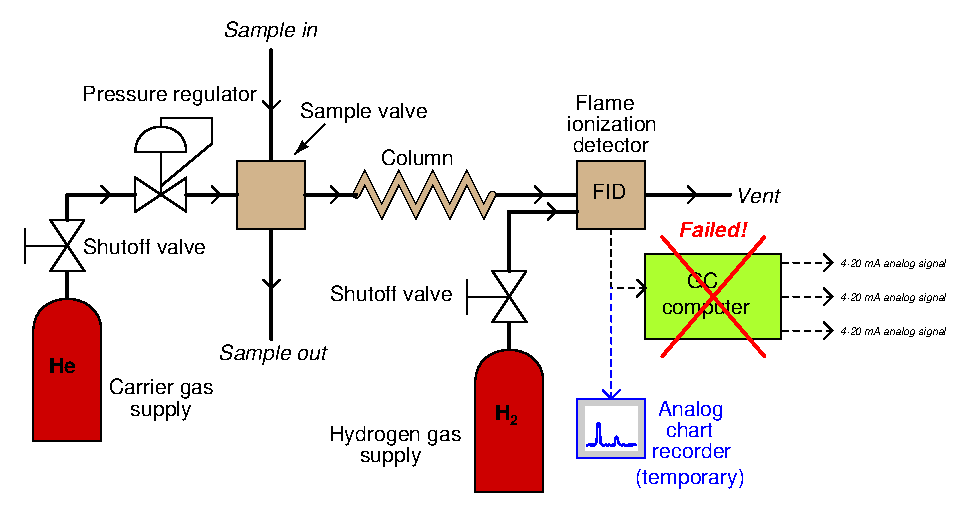
\includegraphics[width=15.5cm]{i01121x01.eps}$$

The technician figures we will still be able to obtain reasonable estimates of species concentration by graphically measuring the area enclosed by each of the peaks plotted on the recorder chart paper, allowing continued operation of this important instrument until a replacement computer arrives from the manufacturer.  If one of the chromatogram peaks measures out to have twice the geometric area of another, he figures, we will know that species' concentration is twice that of the other species.  Defending the idea, the technician says, ``I realize I won't be able to measure concentration to the same degree of precision and accuracy as the computer can, but at least I'll be able to tell the relative concentrations -- whether or not one species is more prevalent than another -- just by seeing which peaks have more area than others.''

\vskip 10pt

Explain what is fundamentally flawed about this idea, as clever as it may be.  Then, give one practical example illustrating how the technician's strategy will lead to incorrect measurements of concentration.

\underbar{file i01121}
%(END_QUESTION)





%(BEGIN_ANSWER)

5 points for reason, 5 points for example:
 
\vskip 10pt

The reason this idea won't work has to do with {\it response factor}.  The detector (in this case an FID) does not respond with equal sensitivity to all the different species.  This inequality of response renders the technician's approach of ``apples-to-apples'' peak area comparison impractical.

\vskip 10pt

Two peaks may have the exact same geometric area, yet represent substantially different concentration levels of hydrocarbon, simply because the detector responds with greater sensitivity to one of those compounds than the other.  For example, we know that an FID responds proportionately to the amount of carbon in the molecule.  A ``C12'' molecule will generate a stronger signal (i.e. a bigger peak) from the FID than a ``C10'' molecule, even if the concentrations of each species are precisely equal.

%(END_ANSWER)





%(BEGIN_NOTES)

{\bf This question is intended for exams only and not worksheets!}.

%(END_NOTES)


